\graphicspath{{../../S25_Distributivite_simple_et_egalites/Images/}}

\themeN
\chapter{Distributivité simple et égalités}
\label{S25}

\programme%
   {\item Propriétés de distributivité simple.}
   {\item Développer, factoriser, réduire des expressions littérales dans des cas très simples.}

\vfill

\begin{debat}{Débat : polysémie du facteur}
   La {\bf polysémie} est la caractéristique d'un mot ou d'une expression qui a plusieurs sens ou significations différentes. En mathématiques, on utilise régulièrement des mots qui n'ont pas forcément le même sens qu'en français par exemple. \par
   Le mot {\bf facteur} ne déroge pas à cette règle : étymologiquement, il vient du latin {\it factir}, celui qui fait. Le facteur que nous utilisons en mathématiques désigne un terme d'un produit, et le facteur que nous connaissons le mieux est certainement la personne distribuant le courrier. À l'origine, le facteur est un fabriquant d'instruments de musique. Enfin, le terme facteur s'utilise aussi en économie ou en biologie pour mentionner un élément important qui concourt à un résultat.
   \tcblower
      \begin{pspicture}(0,0)(3,2)
         \psframe[fillstyle=solid,fillcolor=DodgerBlue!25](0,0)(3,2)
         \pspolygon[fillstyle=solid,fillcolor=DodgerBlue!20](0,2)(1.5,0.8)(3,2)
      \end{pspicture}
\end{debat}

\hfill {\gray Vidéo : \href{https://www.youtube.com/watch?v=g73sqrZZlQo}{\bf Comprendre la simple distributivité}, chaîne YouTube de {\it Jean-Yves Labouche}.}


%%% Approche %%%
\begin{Maquette}[Cours]{Theme={Activité d'approche},Couleur={SteelBlue}}

   \AAtitre{Je veux du chocolat !}

   {\it Objectifs : découvrir la distributivité simple pour réduire une expression littérale de la forme $ax+bx$ où $a$ et $b$ sont des nombres décimaux.}

      \begin{AActivite}

         Un chocolatier expérimente une nouvelle tablette de chocolat pour son magasin : celle-ci est composée de rangées de chocolat dont le cacao vient de côte d'ivoire (CI) et d'un tout nouveau chocolat du Brésil (BR), un peu plus clair. Sa tablette représentée ci-dessous est composée de \Masse{64} de chocolat CI et de \Masse{32} de chocolat BR.
         \begin{center}
            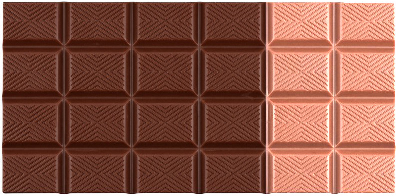
\includegraphics[width=5.25cm]{chocolat}
         \end{center}
         \begin{enumerate}
            \item Il fait un premier test sur 20 tablettes de chocolat qu'il distribue à ses amis pour la tester. \par
               Combien a-t-il besoin de chocolat en tout : trouver deux manières de calculer la masse des 20 tablettes et écrire les deux calculs {\it (aide : on peut utiliser des parenthèses dans l'un des calculs)}. \par \medskip
               Calcul 1 : \pointilles  \par \bigskip
               Calcul 2 : \pointilles \smallskip
            \item Ses amis trouvent qu'il n'y a pas de chocolat BR, ils proposent donc un deuxième test sur 35 tablettes de chocolat, mais en utilisant cette fois-ci \Masse{56} de chocolat CI et \Masse{40} de chocolat BR. \par
               Combien a-t-il besoin de chocolat en tout ?  \par \medskip
               Calcul 1 : \pointilles  \par \bigskip
               Calcul 2 : \pointilles \smallskip
            \item Pour pouvoir effectuer ses calculs plus rapidement, il décide de trouver une formule littérale qui lui permette de calculer le nombre de carreaux de chocolat dont il aura besoin. \par
               \begin{minipage}{8cm}
                  On note :
                  \begin{itemize}
                     \item $a$ le nombre de rangées de chocolat CI ;
                     \item $b$ le nombre de rangées de chocolat BR ;
                     \item $x$ le nombre de lignes de chocolat.
                  \end{itemize}
               \end{minipage}
               \qquad
               \begin{minipage}{7cm}
                  \psset{xunit=0.75,yunit=0.525}
                  \begin{pspicture}[subgriddiv=0,gridlabels=0,gridcolor=gray](-3,-0.8)(6,4.8)
                     \psgrid(0,0)(6,4)
                     \psframe[linewidth=0.5mm](0,0)(6,4)
                     \psline[linewidth=0.5mm](4,0)(4,4)
                     \psline[linecolor=marron]{<->}(-0.3,0)(-0.3,4)
                     \rput(-0.6,1.5){\textcolor{marron}{$x$}}
                     \psline[linecolor=marron]{<->}(0,4.4)(4,4.4)
                     \rput(2,4.8){\textcolor{marron}{$a$}}
                     \psline[linecolor=marron]{<->}(4,4.4)(6,4.4)
                     \rput(5,4.8){\textcolor{marron}{$b$}}
                  \end{pspicture}
               \end{minipage}
               \begin{enumerate}
               \item Donner deux expressions littérales permettant de calculer le nombre total de carreaux de chocolat.  \par \smallskip
                  Calcul 1 : \pointilles  \par \medskip
                  Calcul 2 : \pointilles \smallskip
               \item Sachant que le nombre de carreaux est le même dans les deux expressions, écrire l'égalité qui résulte de ces deux calculs. \par \smallskip
                  \pointilles
            \end{enumerate}
         \end{enumerate}

      \end{AActivite}

\end{Maquette}


%%%Trace écrite %%%
\begin{Maquette}[Cours]{Theme={Trace écrite},Couleur={0.4[SteelBlue,Black]}}

   %%%1
   \section{Réduire une expression littérale}

      \begin{propriete*}{}
         Soit $x$ une variable et $a$ et $b$ des nombres décimaux, 
         \begin{center}
            $a\times x+b\times x =(a+b)\times x \qquad \text{ou} \qquad ax+bx =(a+b)x$ \par
            $a\times x-b\times x =(a-b)\times x \qquad \text{ou} \qquad ax-bx =(a-b)x$
         \end{center}
         On dit qu'on a réduit l'expression littérale.
      \end{propriete*}
      
      \begin{center}
         {\psset{unit=0.6}
         \begin{pspicture}(0,0.5)(7.3,2.5)
            \psframe(0,0)(5,2)
            \psline(3.5,0)(3.5,2)
            \rput(1.75,1){$ax$}
            \rput(4.25,1){$bx$}
            \psline[linecolor=Crimson]{<->}(-0.2,0)(-0.2,2)
            \rput(-0.5,1){\textcolor{Crimson}{$x$}}
            \psline[linecolor=DodgerBlue]{<->}(0,2.2)(3.5,2.2)
            \rput(1.75,2.5){\textcolor{DodgerBlue}{$a$}}
            \psline[linecolor=DodgerBlue]{<->}(3.5,2.2)(5,2.2)
            \rput(4.25,2.5){\textcolor{DodgerBlue}{$b$}}
            \rput(6,1){\Large =}
         \end{pspicture}
         \begin{pspicture}(0,0.5)(5,2.5)
            \psframe(0,0)(5,2)
            \rput(2.5,1){$(a+b)x$}
            \psline[linecolor=Crimson]{<->}(-0.2,0)(-0.2,2)
            \rput(-0.5,1){\textcolor{Crimson}{$x$}}
            \psline[linecolor=DodgerBlue]{<->}(0,2.2)(5,2.2)
            \rput(2.5,2.5){\textcolor{DodgerBlue}{$a+b$}}
         \end{pspicture}}
      \end{center}
      
      \begin{exemple*}{}
         \begin{itemize}
            \item $8\times\textcircledd{x}+3\times\textcircledd{x} =(8+3)\times\textcircledd{x} =11\times\textcircledd{x} =11x$.
            \item $12\,\textcircledd{n}-7\,\textcircledd{n} =(12-7)\,\textcircledd{n} =5\,\textcircledd{n} =5n$.
         \end{itemize}
      \end{exemple*}
      
      
   %%%2
   \section{Utiliser la distributivité pour calculer}
      
      Ces différentes formes nous permettent de d'effectuer des calculs plus facilement.
      
      \begin{center}
         \begin{pspicture}(0,0.6)(8,2.6)
            \psset{nodesep=2mm}
            \rput(4,1.5){\large$ax\rnode{a}+bx = (a\rnode{b}+b)x$} 
            \nccurve[angleA=90,angleB=90,linecolor=DodgerBlue]{->}{a}{b}
            \rput(4,2.6){\textcolor{DodgerBlue}{factoriser}}
            \rput(9,1.7){\textcolor{DodgerBlue}{transformer un produit en somme}}
            \rput(9,1.3){\textcolor{DodgerBlue}{(on a mis les parenthèses)}}
            \nccurve[angleA=-90,angleB=-90,linecolor=Crimson]{->}{b}{a}
            \rput(4,0.4){\textcolor{Crimson}{développer}}
            \rput(-1,1.3){\textcolor{Crimson}{transformer une somme en produit}}
            \rput(-1,1.7){\textcolor{Crimson}{(on a enlevé les parenthèses)}}
         \end{pspicture}
      \end{center}
      
      \begin{exemple*}{}
         \begin{itemize}
            \item $\textcircledd{57}\times28-\textcircledd{57}\times18 =\textcircledd{57}\times(28-18) =\textcircledd{57}\times 10 =570$. 
            \item $13\times102 =\textcircledd{13}\times(100+2) =\textcircledd{13}\times100+\textcircledd{13}\times2 =1\;300+26 = 1\;326$. 
         \end{itemize}
      \end{exemple*}
         
      
   %%%3
   \section{Tester une égalité}
      
      Lorsque l'on choisit une certaine valeur pour chaque lettre d'une expression littérale, on peut en calculer la valeur. 
      
      \begin{exemple*}{}
         Calculer $4\times x+3\times y$ pour $x=5$ et $y =0$ : \par
         $4\times\textcircledd{x}+3\times\textcircledd{y} =4\times\textcircledd{5}+3\times\textcircledd{0} =20+0 =20$.
      \end{exemple*}
      
      Tester une égalité entre deux expressions signifie remplacer les lettres de ces expressions par des valeurs et regarder si les deux membres donnent le même résultat, ou pas !   
      
      \begin{exemple*}{}
         Tester l'égalité $2x+1 =5x-5$ pour $x =3$ et $x =2$.
         \begin{multicols}{2}
            Pour $x =3$, on a : \par
            \begin{itemize}
               \item $2\textcircledd{x}+1 =2\times\textcircledd{3}+1 =7.$
               \item $5\textcircledd{x}-5 =5\times\textcircledd{3}-5 =10.$
            \end{itemize}
            Les deux membres de l'égalité ne sont pas égaux, donc l'égalité n'est pas vraie pour $x=3$. \par
            Pour $x =2$, on a : \par
            \begin{itemize}
               \item $2\textcircledd{x}+1 =2\times\textcircledd{2}+1 =5$.
               \item $5\textcircledd{x}-5 =5\times\textcircledd{2}-5 =5$.
            \end{itemize}
            Les deux membres de l'égalité sont égaux, donc l'égalité est vraie pour $x=2$.
         \end{multicols}
      \end{exemple*}

\end{Maquette}


%%% Exercices %%%
\begin{Maquette}[Fiche,CorrigeFin,Colonnes=2]{}
   
   \begin{multicols}{2}

      \begin{exercice}[SLF] %1
         Réduire chacune des expressions suivantes.
         \begin{enumerate}
            \item $6\times x+6,1\times x =\pointilles$
            \item $3,2g+4,3g =\pointilles$
            \item $8p-4p =\pointilles$
            \item $6\times a+5\times a-7\times a =\pointilles$
            \item $5,8n-2,8n+5,3n-1,1n =\pointilles$ 
         \end{enumerate}
      \end{exercice}
      
      \begin{Solution}
         \begin{enumerate}
            \item $6\times\textcircledd{x}+16\times\textcircledd{x} =(6+16)\times\textcircledd{x} =\cor{22x}$
            \item $3,2\,\textcircledd{g}+4,3\,\textcircledd{g} =(3,2+4,3)\,\textcircledd{g} =\cor{7,5g}$
            \item $8\,\textcircledd{p}-4\,\textcircledd{p} =(8-4)\,\textcircledd{p} =\cor{4p}$
            \item $6\times\textcircledd{a}+5\times\textcircledd{a}-7\times\textcircledd{a} =(6+5-7)\times\textcircledd{a} =\cor{4a}$
            \item $5,8\,\textcircledd{n}-2,8\,\textcircledd{n}+5,3\,\textcircledd{n}-1,1\,\textcircledd{n}$ \par
               $=(5,8-2,8+5,3-1,1)\,\textcircledd{n} =\cor{7,2n}$
         \end{enumerate}
      \end{Solution}
      
      
      \begin{exercice}[SLF] %2
         Entourer le facteur commun de chaque expression, la réduire puis calculer mentalement.
         \begin{enumerate}
            \item $83\times72+83 \times28 =\pointilles$
            \item $36 \times25-36\times5 =\pointilles$
            \item $98\times26+98\times4 =\pointilles$
            \item $16\times44-6\times44 =\pointilles$
         \end{enumerate}
      \end{exercice}
      
      \begin{Solution}
         \begin{enumerate}
            \item $\textcircledd{83}\times72+\textcircledd{83} \times28 =\textcircledd{83}\times(72+28)$ \par
               $=83\times100 =\cor{\num{8300}}$.
            \item $\textcircledd{36}\times25-\textcircledd{36}\times5 =\textcircledd{36}\times(25-5)$ \par
               $=36\times20 =\cor{720}$.
            \item $\textcircledd{98}\times26+\textcircledd{98}\times4 =\textcircledd{98}\times(26+4)$ \par
               $=98\times30 =\cor{\num{2940}}$.
            \item $16\times\textcircledd{44}-6\times\textcircledd{44} =(16-6)\times\textcircledd{44}$ \par
               $=10\times44 =\cor{440}$
         \end{enumerate}
      \end{Solution}
      
      
      \begin{exercice} %3
         On considère l'expression suivante : \par
         $A=97\times27+3\times27$
         \begin{enumerate}
            \item En respectant les priorités opératoires, effectuer le calcul de $A$ sans calculatrice.
            \item Factoriser $A$ puis calculer sa valeur toujours sans calculatrice. Que constate-t-on ?
            \item Calculer sans calculatrice $B =47\times\num{1215}-47\times215$.
         \end{enumerate}
      \end{exercice}  
      
      \begin{Solution}
         \begin{enumerate}
            \item $A=97\times27+3\times27 =\num{2619}+81 =\cor{\num{2700}}$.
            \item $A=97\times\textcircledd{27}+3\times\textcircledd{27} =(97+3)\times\textcircledd{27}$ \par
               $=100\times27 =\cor{\num{2700}}$. \par
               \cor{La méthode  est plus simple et plus rapide}. 
            \item $B =\num{1215}\times\textcircledd{47}-\textcircledd{47}\times215$ \par
               $=\textcircledd{47}\times(\num{1215}-215) =47\times\num{1000} =\cor{\num{47000}}$
         \end{enumerate}
      \end{Solution}  
      
      \begin{exercice} %4
         Développer chaque expression puis calculer.
         \begin{colenumerate}
            \item $5\times(3+9)$
            \item $3\times(10+7)$
            \item $(11-5)\times7$
            \item $2\times(13-4)$
         \end{colenumerate}
      \end{exercice}
      
      \begin{Solution}
         \begin{enumerate}
            \item $\textcircledd{5}\times(3+9) =\textcircledd{5}\times3+\textcircledd{5}\times9 =15+45 =\cor{60}$
            \item $\textcircledd{3}\times(10+7) =\textcircledd{3}\times10+\textcircledd{3}\times7 =30+21 =\cor{51}$
            \item $(11-5)\times\textcircledd{7} =11\times\textcircledd{7}-5\times\textcircledd{7} =77-35 =\cor{42}$
            \item $\textcircledd{2}\times(13-4) =\textcircledd{2}\times13-\textcircledd{2}\times4 =26-8 =\cor{18}$
         \end{enumerate}
      \end{Solution}
      
      
      \begin{exercice} %5
         Parmi les deux méthodes suivantes pour calculer $33\times103$, quelle est la plus rapide ?
         \begin{enumerate}
            \item Poser le calcul en colonnes.
            \item Décomposer le nombre 103 comme la somme de deux nombres simples, puis développer l'expression $33\times(\pointilles[5mm]\,+ \pointilles[5mm]\,)$ obtenue. Que remarque-t-on ?
         \end{enumerate}
      \end{exercice}
      
      \begin{Solution}
         \begin{enumerate}
            \item On trouve $33\times103 =\cor{\num{3399}}$
            \item $\textcircledd{33}\times103 =\textcircledd{33}\times(100+3) =\textcircledd{33}\times100+\textcircledd{33}\times3$ \par
               $=\num{3300}+99 =\cor{\num{3399}}$. \par
               \cor{La deuxième méthode est plus simple pour calculer le résultat de tête}.
         \end{enumerate}
      \end{Solution}
      
      
      \begin{exercice} %6
         On a : $197\times17 =\num{3349}$ et $197\times4 =788$. \par
         Calculer les nombres suivants en proposant une décomposition qui utilise les égalités ci-dessus.
         \begin{colenumerate}
            \item $197\times21$
            \item $197\times13$
            \item $197\times34$
         \end{colenumerate}
      \end{exercice}
      
      \begin{Solution}
         \begin{enumerate}
            \item $197\times21 =197\times(17+4) $\par
               $=197\times17+197\times4 =\num{3349}+788 =\cor{\num{4137}}$
            \item $197\times13 =197\times(17-4)$ \par
               $=197\times17-197\times4 =\num{3349}-788 =\cor{\num{2561}}$
            \item $197\times34 =197\times(17\times2)$ \par
               $=(197\times17)\times2 =3\,349\times2 =\cor{\num{10047}}$
         \end{enumerate}
      \end{Solution}
      
      
      \begin{exercice} %7
         L'égalité $5x =2x+15$ est-elle vérifiée :
         \begin{colenumerate}
            \item Pour $x =4$.
            \item Pour $x =5$.
         \end{colenumerate}
      \end{exercice}
      
      \begin{Solution}
         \begin{enumerate}
            \item $5x =5\times4 =20$ et $2x+15 =2\times4+15 =23$. \par
               donc, pour $x =4$, \cor{l'égalité n'est pas vérifiée}.
            \item $5x =5\times5 =25$ et $2x+15=2\times5+15 =25$. \par
               donc, pour $x =5$, \cor{l'égalité est vérifiée.}
         \end{enumerate}
      \end{Solution}
      
      
      \begin{exercice} %8
         \begin{enumerate}
            \item Montrer que l'égalité $2x^2 =6x$ est vraie pour $x =3$.
            \item Peut-on trouver un autre nombre pour lequel l'égalité précédente est vérifiée ?
         \end{enumerate}
      \end{exercice}
      
      \begin{Solution}
         \begin{enumerate}
            \item $2x^2 =2\times3^2 =18$ et $6x =6\times3 =18$. \par
            donc, pour $x =3$, \cor{l'égalité est vérifiée}.
            \item $2x^2 =2\times0^2 =0$ et $6x =6\times0 =0$. \par
            donc, \cor{pour $x =0$} l'égalité est encore vérifiée.
         \end{enumerate}
      \end{Solution}
      
      
      \begin{exercice} %9
         Déterminer si l'égalité $3y =4x-3$ est vérifiée :
         \begin{colenumerate}
            \item pour $y =3$ et $x =3$.
            \item pour $y =2$ et $x =4$.
         \end{colenumerate}
      \end{exercice}
      
      \begin{Solution}
         \begin{enumerate}
            \item $3y =3\times3 =9$ et $4x-3 =4\times3-3 =9$. \par
            donc, pour $y =3$ et $x =3$, \cor{l'égalité est vérifiée}.
            \item $3y =3\times2 =6$ et $4x-3 =4\times4-3 =13$. \par
            pour $y =2$ et $x =4$, \cor{l'égalité n'est pas vérifiée}.
         \end{enumerate}
      \end{Solution}
      
      
      \begin{exercice}[Dur] %10
         Dans les trois tours de magie suivants, on demande à une personne d'effectuer des calculs mentalement. \par
         Chercher comment il est possible de retrouver le nombre pensé à partir du résultat. \par \smallskip
         {\bf Tour 1}
         \ProgCalcul[Enonce,Largeur=6cm]{Choisir un nombre,Ajouter 1, Doubler le résultat,Retrancher 2,Donner son résultat}
         {\bf Tour 2}
         \ProgCalcul[Enonce,Largeur=6cm]{Choisir un nombre,Ajouter 1, Doubler le résultat,Ajouter 1,Retrancher le nombre pensé,Donner son résultat}
         {\bf Tour 3}
         \ProgCalcul[Enonce,Largeur=6cm]{Choisir un nombre,Enlever 1,Doubler le résultat,Enlever 1,Ajouter au résultat le nombre pensé,Donner son résultat}   
      \end{exercice}
      
      \begin{Solution}
         {\bf Tour 1}
         {\small
            \ProgCalcul[Application,SansCalcul]{Ajouter 1, Doubler le résultat,Retrancher 2
            §
            n,+1 *2 -2 ,n+1 2\times(n+1)=2n+2 2n+2-2=2n}}
         Le résultat donné est le double du nombre choisi. \cor{Il suffit donc de prendre la moitié du résultat donné}. \par \smallskip
         {\bf Tour 2}
         {\small
            \ProgCalcul[Application,SansCalcul]{Ajouter 1, Doubler le résultat,Ajouter 1,Retrancher le nombre pensé
            §
            n,+1 *2 +1 -n,n+1 2\times(n+1)=2n+2 2n+2+1=2n+3 2n+3-n=n+3}}
         Le résultat donné est le nombre choisi, augmenté de 3. \cor{Il suffit donc de soustraire 3 au résultat donné}. \par \smallskip
         {\bf Tour 3}
         {\small
            \ProgCalcul[Application,Largeur=8cm,SansCalcul]{Enlever 1,Doubler le résultat,Enlever 1,Ajouter au résultat le nombre pensé,
            §
            n,-1 *2 -1 +n,n-1 2\times(n-1)=2n-2 2n-2-1=2n-3 2n-3+n=3n-3}}
         Le résultat donné est le triple du nombre choisi, diminué de 3. \cor{Il suffit donc d'ajouter 3 au résultat donné, puis de le diviser par 3}.
      \end{Solution}
         
   \end{multicols}

\end{Maquette}


%%% Récré %%%
\begin{Maquette}[Cours]{Theme={Activité récréative},Couleur={IndianRed}}
    
   \ARtitre{Un diamant littéral}
      \begin{minipage}{9cm}
         Découper les douze pièces du puzzle et les assembler de telle sorte que les expressions face à face soient égales. \par
         Coller le puzzle sur votre cahier. \par
         La forme à obtenir est celle ci-contre.
      \end{minipage}
      \hfill
      \begin{minipage}{5cm}
         {\psset{unit=0.8}
         \begin{pspicture}(0,1)(6,7)      
            \rput{-60}(2,4){\tri{}{}{}}
            \rput(2,4){\tri{}{}{}}
            \rput{60}(2,4){\car{}{}{}{}}
            \rput{150}(2,4){\tri{}{}{}}
            \rput{-150}(2,4){\car{}{}{}{}}
            \rput{-150}(3,2.27){\tri{}{}{}}
            \rput{-90}(3,2.27){\tri{}{}{}}
            \rput{-120}(4,4){\car{}{}{}{}}
            \rput{-30}(4,4){\tri{}{}{}}
            \rput{30}(4,4){\car{}{}{}{}}
            \rput{30}(3,5.73){\tri{}{}{}}
            \rput{90}(3,5.73){\tri{}{}{}}
         \end{pspicture}}
      \end{minipage}
      \begin{center}
         {\psset{unit=2.5,linewidth=0.6mm} \large
         \begin{pspicture}(0,-0.5)(6,6.5)
            \rput(0,0){\car{4x-8x+6x}{14x+35x}{13x}{}} %6
            \rput(2,0){\car{42x}{12x}{}{8x-4x}} %3
            \rput(4,0){\car{25x}{}{20x+8x-5x}{77x}} %5
            \rput(0,2){\tri{}{2x}{20x+5x}} %12
            \rput{60}(2,2){\tri{154x}{7x+70x}{x}} %2
            \rput(2,2){\tri{}{15x}{16x-4x}} %9
            \rput{60}(4,2){\tri{7x+35x}{14x-35x+22x}{49x}} %1
            \rput(4,2){\tri{}{0}{2x+15x-4x}} %7
            \rput(0,3.73){\car{14x+140x}{20x}{}{10x+5x}} %4
            \rput(2,3.73){\tri{4x}{2x-2x}{}} %8
            \rput{60}(4,3.73){\tri{30x}{10x+10x}{}} %10
            \rput(4,3.73){\tri{}{23x}{10x+20x}} %11
         \end{pspicture}}
      \end{center}

   \vfill \hfill{\it\footnotesize Source : inspiré de \href{https://www.monclasseurdemaths.fr/profs/puzzles/}{monclasseurdemaths.fr}}

\end{Maquette}